%====================================================================%
%                  MORIOND.TEX                                       %
%====================================================================%

\documentclass{moriond}

\usepackage{lineno}

% I want to have square brackets
\usepackage[square,numbers]{natbib}

% For subfigures (e.g. (a) and (b))
\usepackage{subfig}

\bibliographystyle{unsrt}    
% for BibTeX - sorted numerical labels by order of
% first citation.

\usepackage{xspace}
\def\wh{\texorpdfstring{\ensuremath{W\kern -0.1em H}\xspace}{WH\xspace}}
\def\wz{\texorpdfstring{\ensuremath{W\kern -0.1em Z}\xspace}{WZ\xspace}}
\def\vh{\texorpdfstring{\ensuremath{V\kern -0.1em H}\xspace}{VH\xspace}}
\def\zh{\ensuremath{ZH}\xspace}
\def\ttbar{\ensuremath{t\bar{t}}\xspace}

% A useful Journal macro
\def\Journal#1#2#3#4{{#1} {\bf #2}, #3 (#4)}

% Some useful journal names
\def\NCA{\em Nuovo Cimento}
\def\NIM{\em Nucl. Instrum. Methods}
\def\NIMA{{\em Nucl. Instrum. Methods} A}
\def\NPB{{\em Nucl. Phys.} B}
\def\PLB{{\em Phys. Lett.}  B}
\def\PRL{\em Phys. Rev. Lett.}
\def\PRD{{\em Phys. Rev.} D}
\def\ZPC{{\em Z. Phys.} C}

% Some other macros used in the sample text
\def\st{\scriptstyle}
\def\sst{\scriptscriptstyle}
\def\mco{\multicolumn}
\def\epp{\epsilon^{\prime}}
\def\vep{\varepsilon}
\def\ra{\rightarrow}
\def\ppg{\pi^+\pi^-\gamma}
\def\vp{{\bf p}}
\def\ko{K^0}
\def\kb{\bar{K^0}}
\def\al{\alpha}
\def\ab{\bar{\alpha}}
\def\be{\begin{equation}}
\def\ee{\end{equation}}
\def\bea{\begin{eqnarray}}
\def\eea{\end{eqnarray}}
\def\CPbar{\hbox{{\rm CP}\hskip-1.80em{/}}}
%temp replacement due to no font
%%%%%%%%%%%%%%%%%%%%%%%%%%%%%%%%%%%%%%%%%%%%%%%%%%
%                                                %
%    BEGINNING OF TEXT                           %
%                                                %
%%%%%%%%%%%%%%%%%%%%%%%%%%%%%%%%%%%%%%%%%%%%%%%%%%

%\newcommand{\Photo}{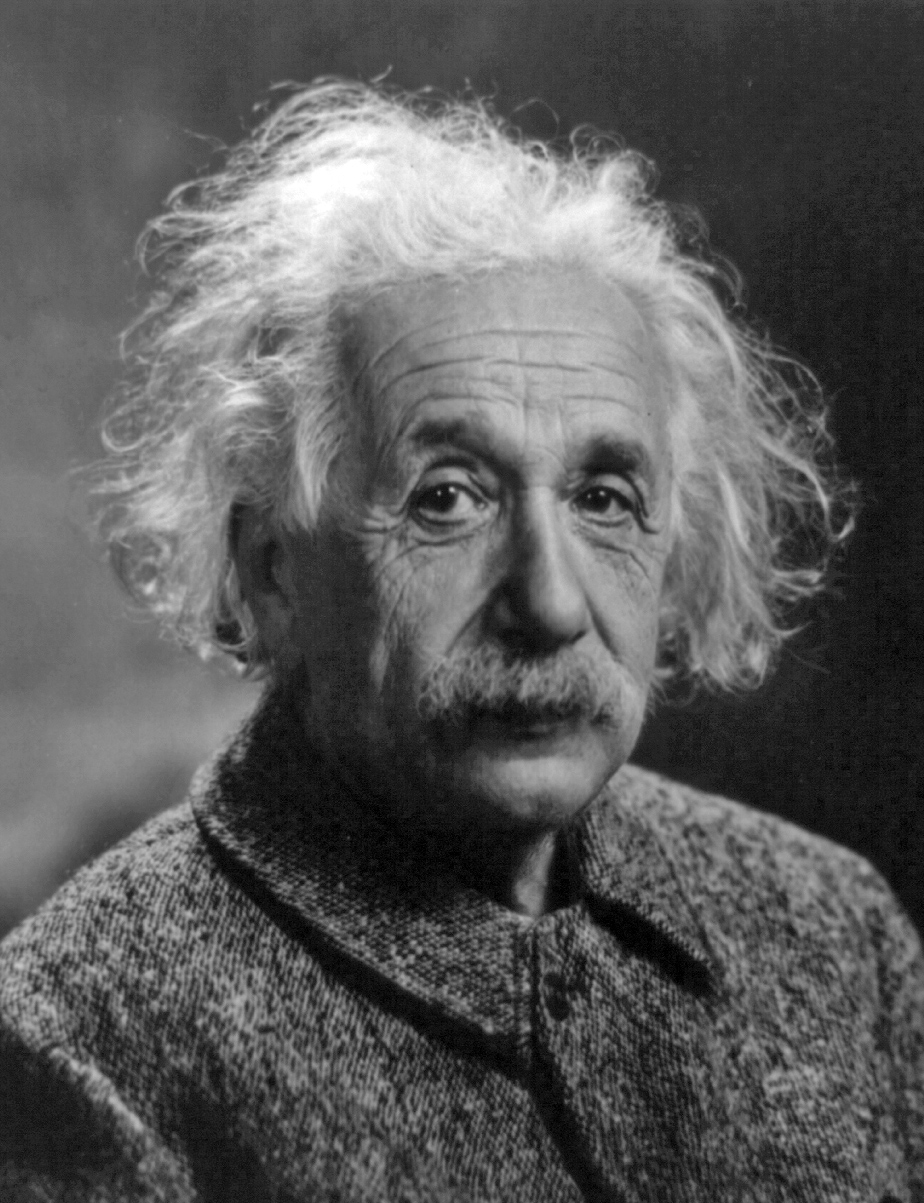
\includegraphics[height=35mm]{mypicture}}
\newcommand{\Photo}{}

\begin{document}
\linenumbers

\vspace*{4cm}
\title{ATLAS Higgs Physics Results}

\author{ Kurt Brendlinger, on behalf of the ATLAS Collaboration }

\address{~\\DESY, Notkestra\ss e 85,\\ 22607 Hamburg, Germany}

\maketitle\abstracts{
Recent Higgs boson results are presented using up to 140~fb$^{-1}$ of proton-proton collision data
delivered by the Large Hadron Collider and recorded by the ATLAS Detector.
Three measurements are discussed:
first, the cross section of a Higgs boson produced in association with a vector boson is measured in phase space
regions called simplified template cross sections (STXS),
using events with the Higgs decaying to a $b\bar b$ pair.
An additional measurement of this associated Higgs production is performed in the $H{\rightarrow}WW$
decay channel.
Finally, the production of a Higgs in association iwth a $t\bar t$ pair is measured in the Higgs
diphoton decay channel. In addition, the status of searches for di-Higgs production is reviewed.
}

\section{Introduction}

The Large Hadron Collider (LHC) \cite{Evans:2008zzb} has delivered about 155 fb$^{-1}$ of
collisions at a center-of-mass energy of $\sqrt{s}=13$~TeV during its Run 2 data taking program
between 2015 and 2018.
With this data, the
ATLAS Detector \cite{PERF-2007-01} is able to probe the nature of the Higgs boson with unprecedented
precision. The following summarizes the most recent measurements of Higgs boson production using up
to 140 fb$^{-1}$ of high-quality data. These measurements are performed in the $b\bar b$,
diphoton ($\gamma\gamma$) and $WW$ (${\rightarrow}\ell\nu\ell'\nu'$) decay channels, and specifically
target Higgs production in association with a vector boson (\vh) or in assoication with a top
quark pair ($t\bar tH$).

Higgs measurements are performed in the context of the simplified template cross section
framework \cite{deFlorian:2016spz,Badger:2016bpw},
which is designed to measure cross sections of production modes as well as kinematic phase space
regions, while reducing the model dependence contained inside the measurements.

\section{Measurement of the \vh production mode in the $b\bar b$ decay channel}\label{sec:vh_bb}

The observation of Higgs boson production in association with a $W$ or $Z$ boson, reported in
\cite{HIGG-2018-04}, was achieved by combined measurements in the $H{\rightarrow}b\bar b$,
$H{\rightarrow}ZZ^*{\rightarrow}4\ell$ and $H{\rightarrow}\gamma\gamma$ decay channels using
80~fb$^{-1}$ of data collected in Run~2.
Following the observation, the \vh production mode is studied in further detail using Higgs bosons
decaying to a pair of $b$-jets \cite{Aaboud:2019nan}, the most sensitive decay channel for the \vh production mode,
using the same analysis strategy and integrated luminosity.
The cross section is measured in bins of the transverse momentum of the associated vector boson,
$p^{V}_\mathrm{T}$. We do this because BLAH.

The analysis considers events with 2 $b$-tagged jets and 0, 1 or 2 reconstructed leptons consistent
with vector boson signatures. To extract the signal, eight separate boosted decision trees (BDTs)
are trained, one for each signal region considered.
The correlation between the $p^{V}_\mathrm{T}$ and the BDT output score is exploited
to extract the cross section in each truth $p^{V}_\mathrm{T}$ category.
Figure~\ref{fig:vh_bb_a} compares the BDT output of the inclusive signal as well as the two
truth categories (?) for a signal region targeting \wh production with the $W$ boson decaying to
$\ell\nu$. The clear shape differences, and their distinguishability from background, can be used to
extract both cross sections simultaneously. The use of a BDT allows for more sensitive cross section
measurements, in the simplified template scheme, than a simple fiducial cross section, because the
improved discrimination against background and between STXS regions.

\begin{figure}[!htbp]
  \centering
  \subfloat[\label{fig:vh_bb_a}] {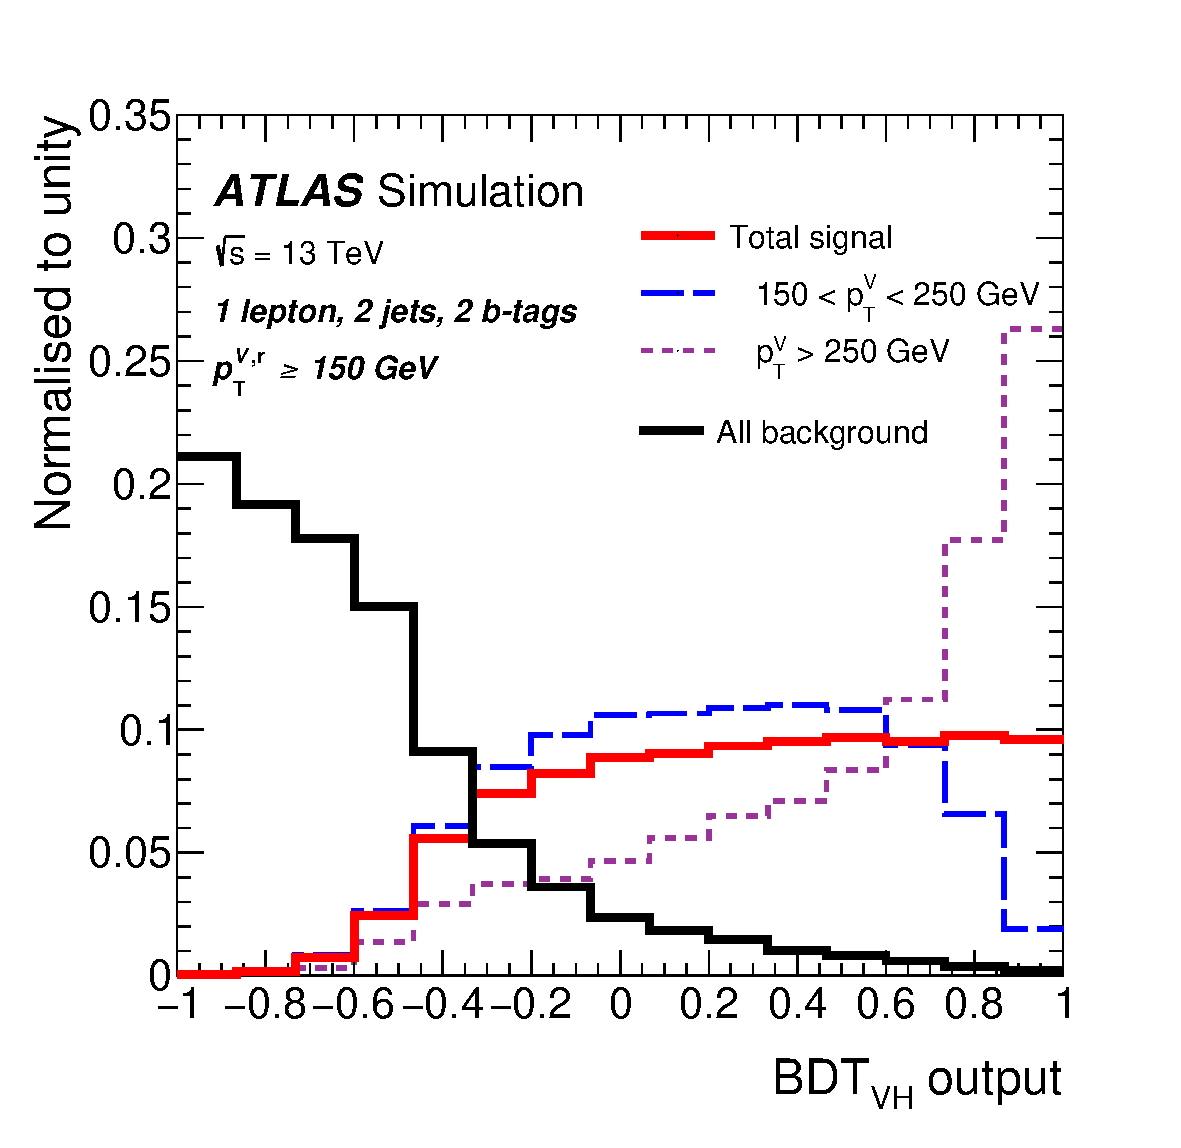
\includegraphics[width=0.425\textwidth]{figures/HIGG-2018-50/fig_01_v1.pdf}}
  \subfloat[\label{fig:vh_bb_b}] {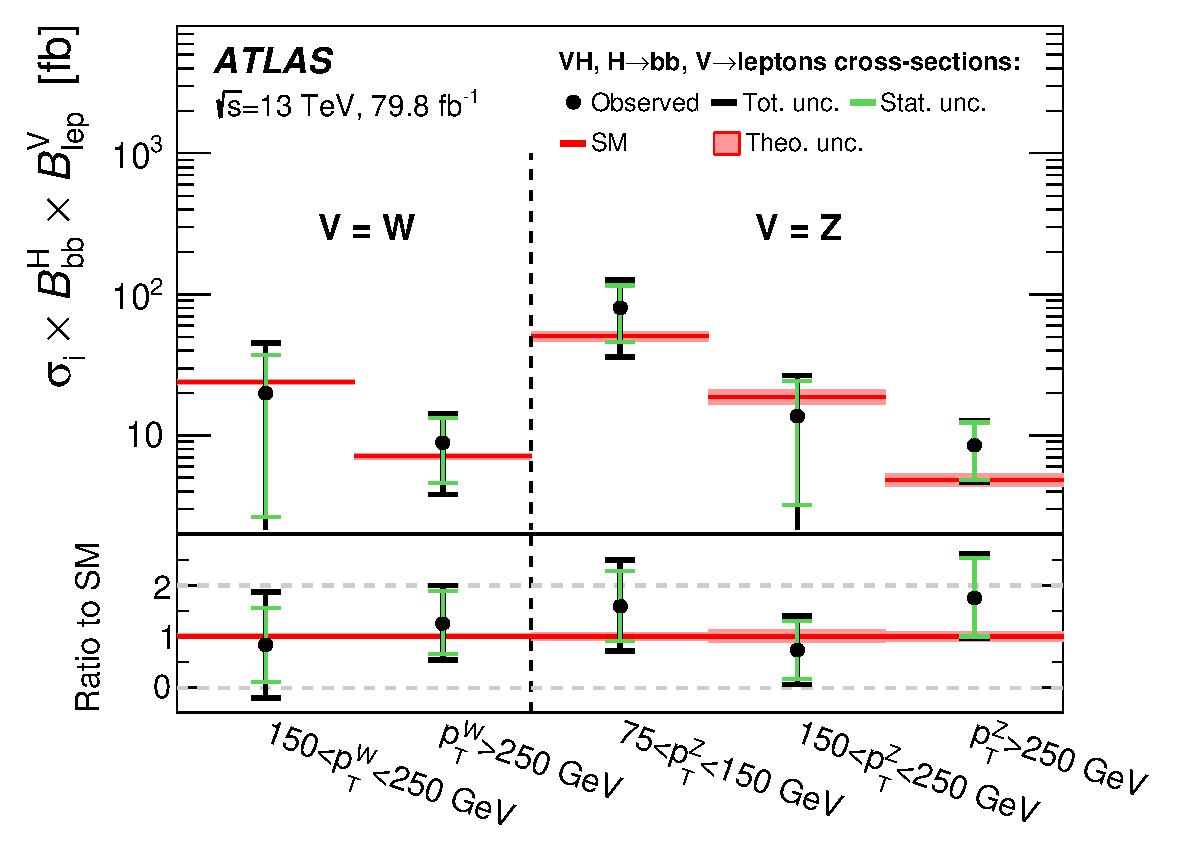
\includegraphics[width=0.565\textwidth]{figures/HIGG-2018-50/fig_03.pdf}}
  \caption{
    (a) The shape of the signal and background  distributions of the BDT in the 1-lepton, 2-jet
    reconstructed event category targeting \wh production. The shape of two STXS signal regions
    featuring different $p^{V}_\mathrm{T}$ is also shown, highlighting the correlation between
    $p^{V}_\mathrm{T}$ and the BDT response.
    (b) The measured cross sections in five STXS regions, and their comparison to the SM prediction  \cite{Aaboud:2019nan}.
  }
  \label{fig:vh_bb}
\end{figure}

Figure~\ref{fig:vh_bb_b} reports the measured cross sections in each of the measured fiducial regions
of the simplified template cross section framework. The measurements presented here are also used
to constrain parameters in an effective Lagrangian framework, such as dimension-6 operators whose
deviation from predictions would indicate interactions beyond the Standard Model. Furthermore, the
simplified template cross sections measured in this analysis can be readily combined with other
decay channels, allowing each decay channel to contribute toward reaching the ultimate precision of
the full Higgs fiducial phase space.

\section{Measurement of the \vh production mode in the $WW$ decay channel} \label{sec:vh_ww}

The \vh production of Higgs bosons is also studied in the $H{\rightarrow}WW$ decay channel, with all
decay products decaying leptonically,
using 36.1~fb$^{-1}$ of data collected in 2015 and 2016 \cite{HIGG-2017-14}.
To gain sensitivity to the \wh process, events with three reconstructed leptons are separated into
a region depleted in $Z$ bosons by requiring that events have no same-flavor, opposite-charge pair,
thus suppressing large background processes involving $Z$ bosons. Two BDTs, one designed to reject
\ttbar events (BDT$_\ttbar$) and one for reducing the \wz background (BDT$_\wz$), are trained for
this region. The signal region is defined by six bins in the two-dimensional space defined by the two
BDTs: three bins of the BDT$_\ttbar$, each of which is subdivided into two BDT$_\wz$ bins.

A separate signal region targeting \wh production is constructed using the remaining three-lepton
events, and a separate BDT is used to separate signal events from \wz/$W\gamma^*$ and $ZZ^*$
backgrounds. Finally, the \zh process is optimized by separating the signal region into events with
one or two same-flavor, opposite-charge pairs.

The \wh and \zh cross sections are extracted using a simultaneous fit of the signal regions and
control regions enhanced in the main analysis backgrounds.
Figure~\ref{fig:ww_vh_a} depicts the fitted \wh signal and background in the 6 bins of the
$Z$-dominated signal region.
Figure~\ref{fig:ww_vh_b} compares the measured cross section times branching ratio for $ZH$ and \wh,
compared to the SM prediction. A mild excess is seen in both cases, though the measured values are
consistent with the SM expectation.

\begin{figure}[!htbp]
  \centering
  \subfloat[\label{fig:ww_vh_a}] {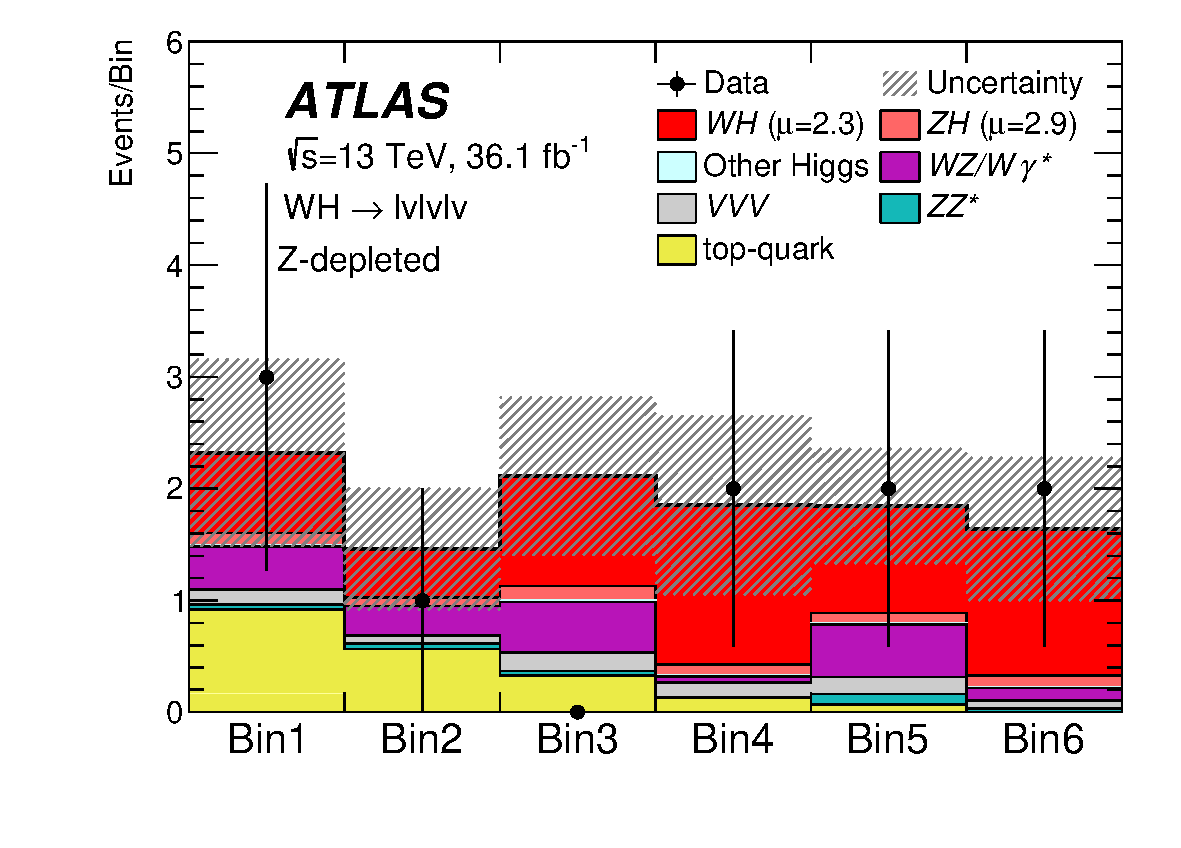
\includegraphics[width=0.55\linewidth]{figures/HIGG-2017-14/fig_06b.pdf}}
  \subfloat[\label{fig:ww_vh_b}] {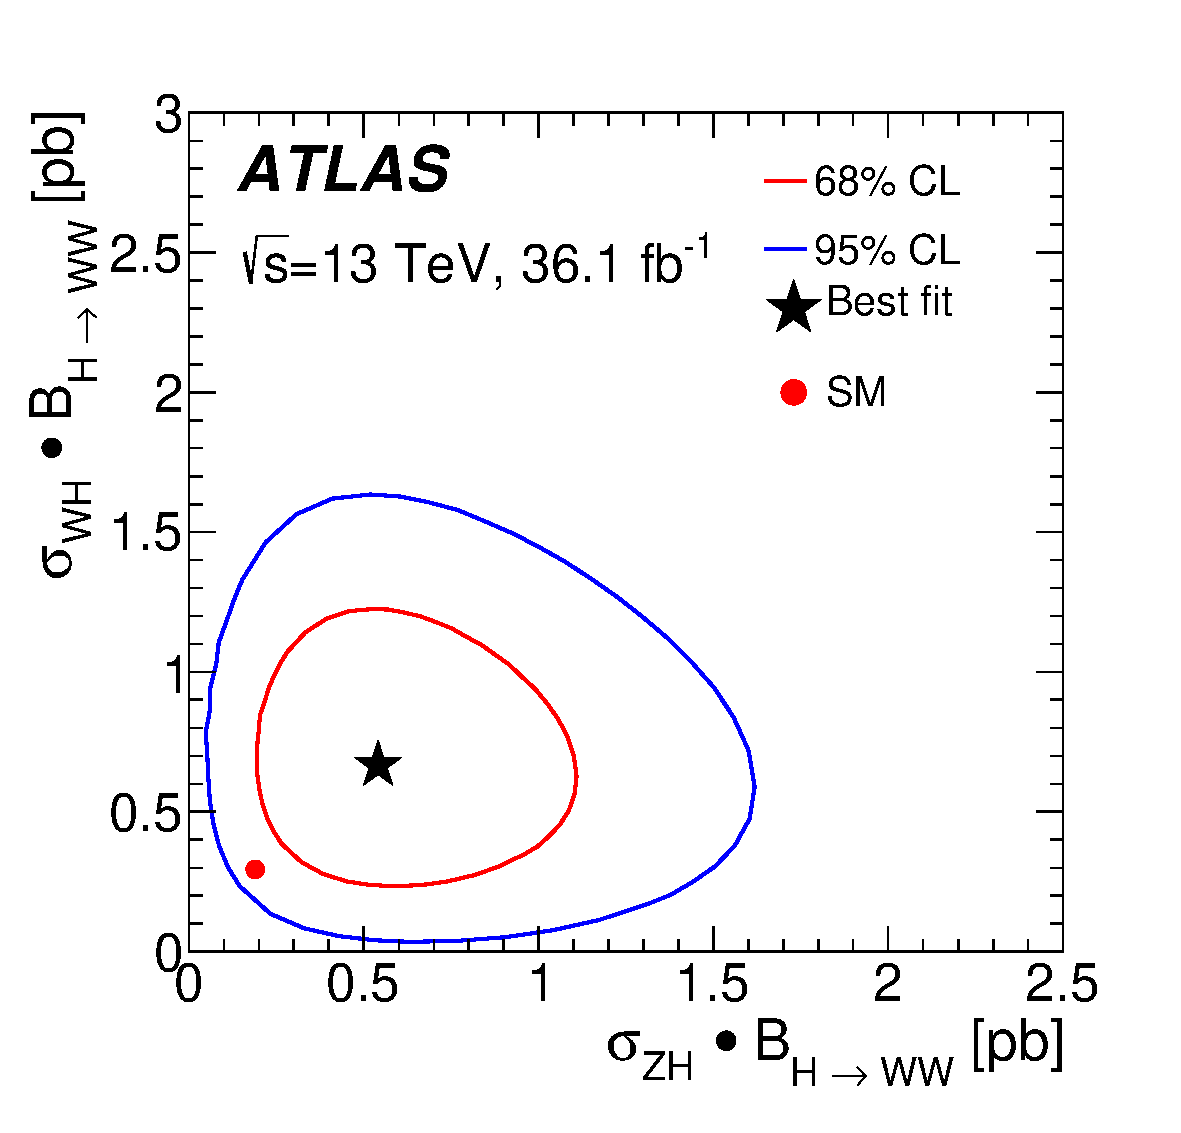
\includegraphics[width=0.44\linewidth]{figures/HIGG-2017-14/fig_08.pdf}}
  \caption{
    (a) The fitted \wh signal and background in the 6 bins most sensitive to \wh production in a
    two-dimensional space defined by the BDT$_{\wz}$ and BDT$_{t\bar t}$ scores---see the text.
    (b) The best-fit cross section times branching ratio for \wh and \zh production and the 68\% and
    95\% confidence level contours, compared to the SM prediction \cite{HIGG-2017-14}.
  }
  \label{fig:ww_vh}
\end{figure}

\section{Measurement of Higgs production in association with a $t\bar t$ pair in the diphoton decay channel}\label{sec:ttH_yy}

The measurement of Higgs production with an associated $t\bar t$ pair ($ttH$ production) and decaying
to two photons has been updated to include the full Run~2 dataset \cite{ATLAS-CONF-2019-004},
following the same analysis strategy as described in \cite{Aaboud:2018urx}. $ttH$ production is
divided into two categories: events with {\itshape hadronic} decays of the $t\bar t$ pair, and
events with {\itshape leptonic} decays of at least one of the top quarks. Two BDTs are developed, one
for hadronic and one for leptonic events, which give discrimination against both non-resonant
background and non-$ttH$ Higgs production. Seven signal regions defined using the BDT scores
(3 BDT bins in the leptonic events and 4 BDTs in the hadronic events) are used to extract the $ttH$
signal.

A simultaneous fit of the invariant diphoton mass spectrm in the 7 BDT categories is performed to
measure the $ttH$ cross section. The $ttH$ signal and non-$ttH$ Higgs production background are
modeled with functions developed from simulated samples, while the continuum background is modeled
with a power law function or an exponential function, chosen separately in each category based on their
performance in data control regions that closely resemble the signal regions.
Figure~\ref{fig:tth_a} shows the sum of she signal and background fits in all 7 categories, where
the contribution from each channel is weighted by its expected significance.

\begin{figure}[!htbp]
  \centering
  \subfloat[\label{fig:tth_a}] {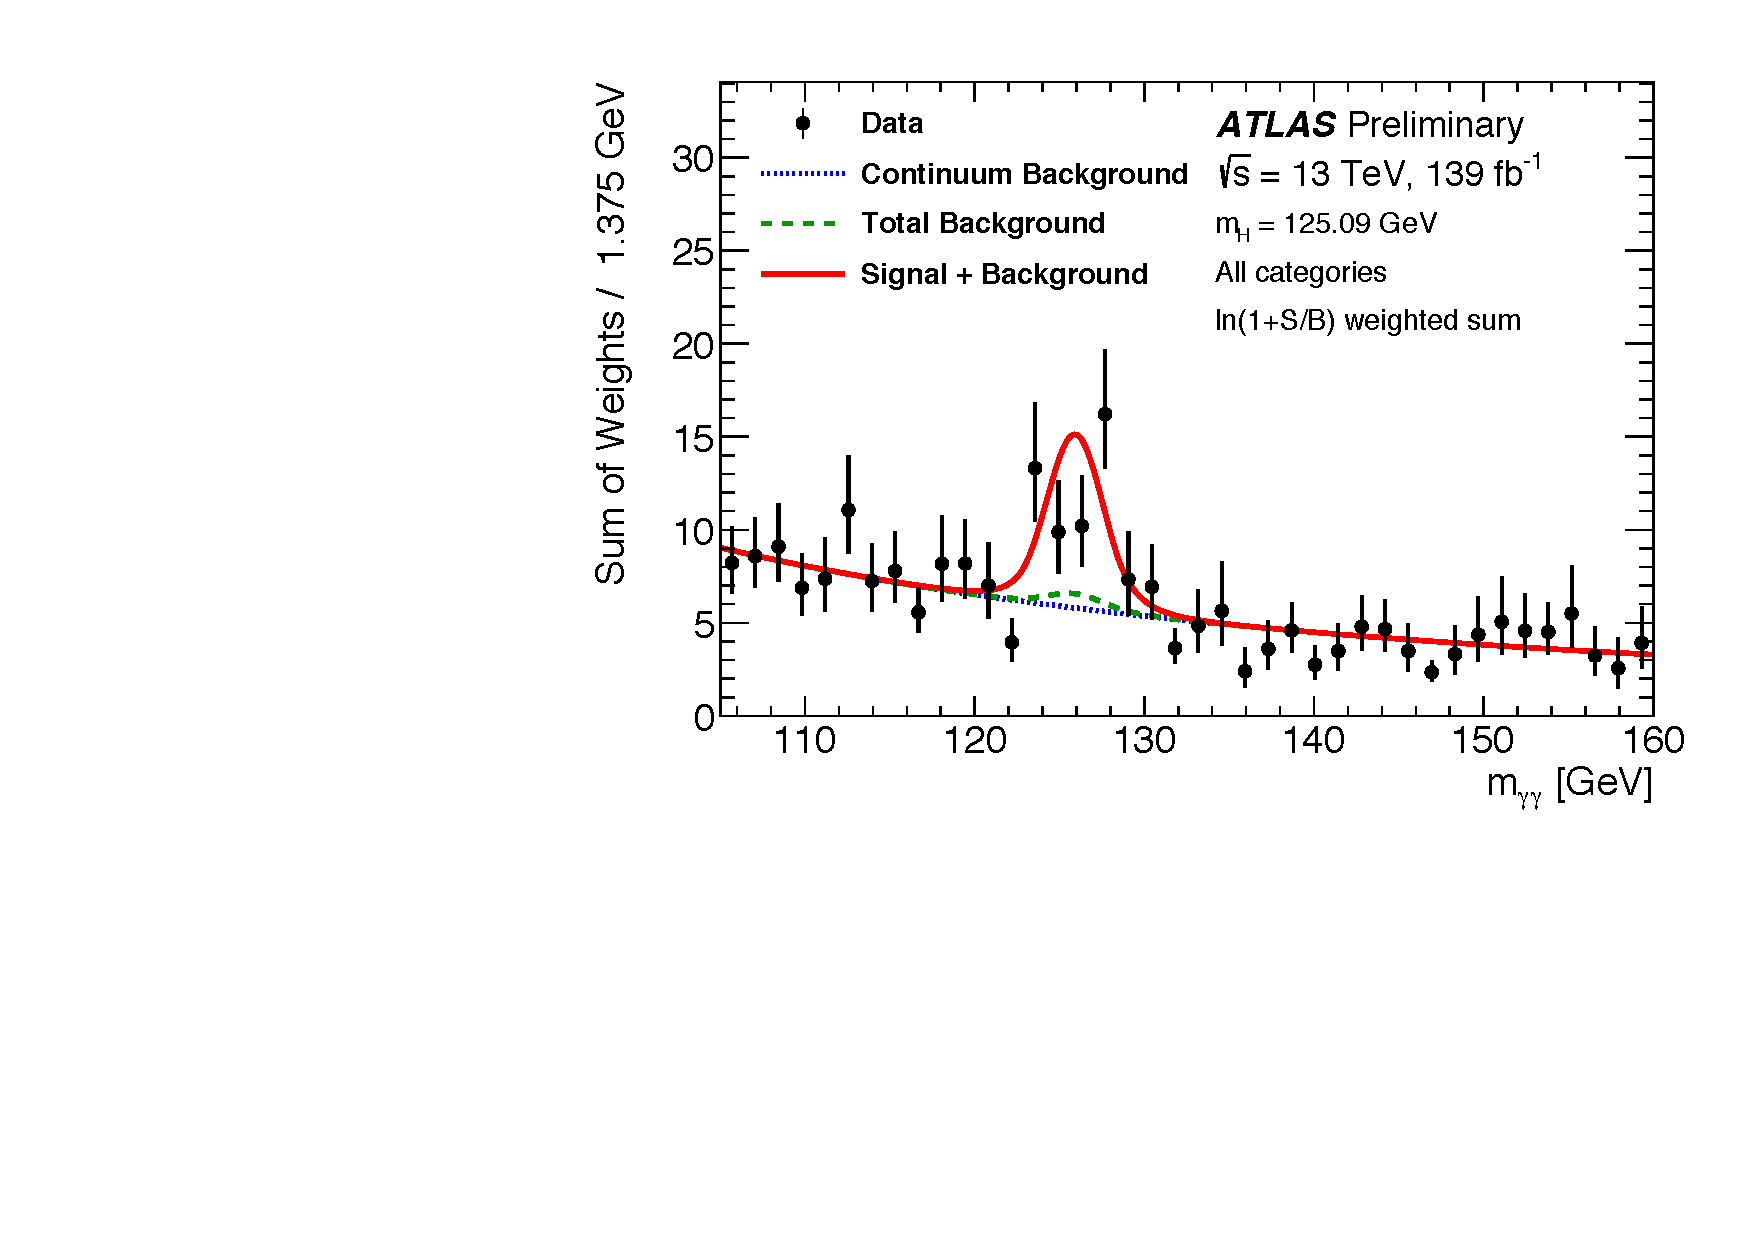
\includegraphics[width=0.525\linewidth]{figures/ATLAS-CONF-2019-004/fig_05_v1.pdf}}
  \subfloat[\label{fig:tth_b}] {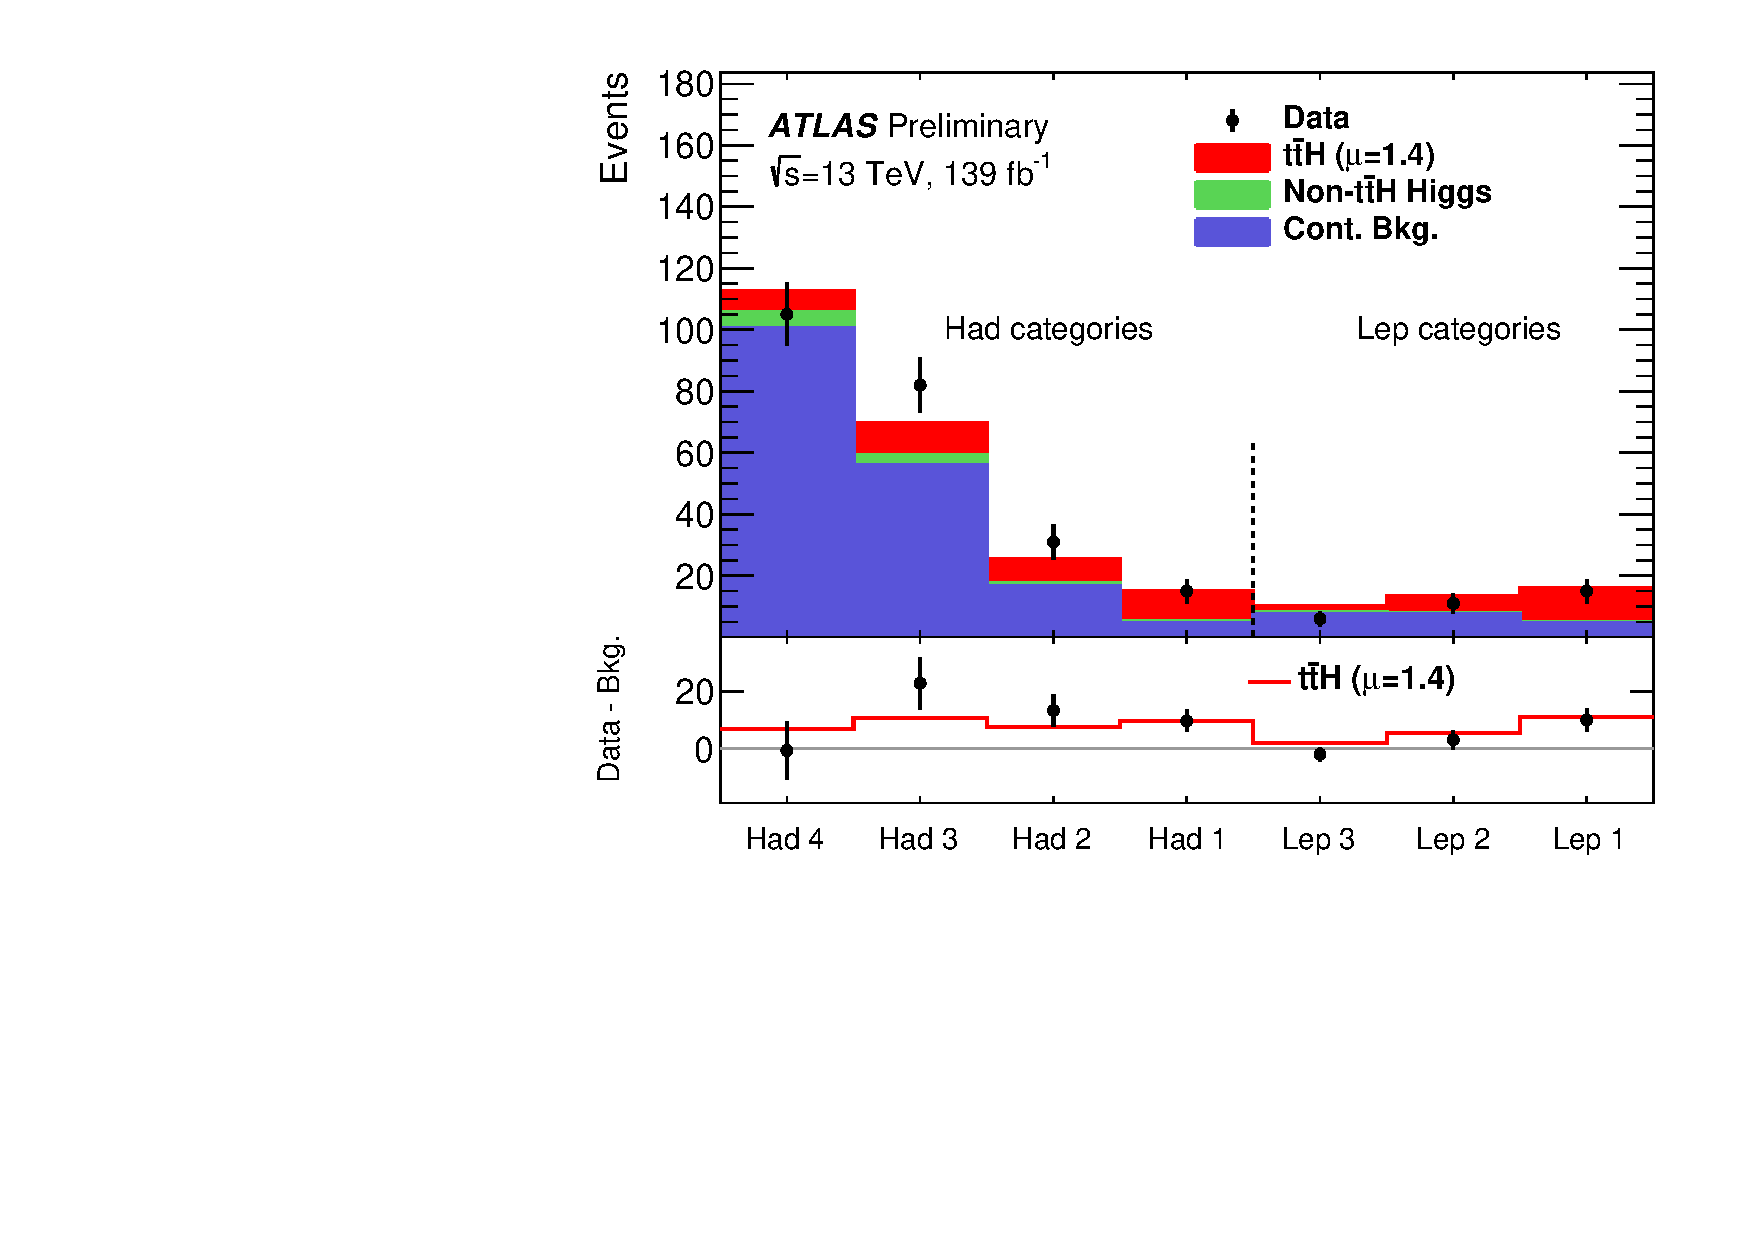
\includegraphics[width=0.465\linewidth]{figures/ATLAS-CONF-2019-004/fig_08.pdf}}
  \caption{
    (a) The invariant mass spectrum of the diphoton system for the sum of all signal regions, weighted
    by the expected significance of each region. The fitted total background includes non-resonant
    backgrounds as well as other (non-$ttH$) Higgs production modes.
    (b) The number of data events in the diphoton invariant mass window containing 90\% of the expected
    $ttH$ signal, in each BDT bin of the hadronic and leptonic categories.
    The fitted $ttH$ signal and background, including continuum backgrounds and non-$ttH$ Higgs
    production, are shown in each bin \cite{ATLAS-CONF-2019-004}.
  }
  \label{fig:tth}
\end{figure}

In Figure~\ref{fig:tth_b}, the contribution of $ttH$ signal, other Higgs
production processes, and continuum background is shown for each category.
The measured $ttH$ production cross section times branching ratio in a fiducial region requiring the
Higgs rapidity $|y_H|<2.5$ is measured to be
%
\begin{equation}
\sigma_{ttH} \times B_{\gamma\gamma} = 1.59~^{+0.38}_{-0.36} ~\textrm{(stat.)}
~^{+0.15}_{-0.12} ~\textrm{(exp.)}
~^{+0.15}_{-0.11} ~\textrm{(th.)}~\textrm{fb},
\end{equation}
%
which is 1.4 times the SM prediction.
The measurement has an observed significance of 4.9$\sigma$ (4.2$\sigma$ expected),
such a high significance
highlights the importance of the diphoton decay channel in the study of $ttH$ production.

%% \section{Limits on the Higgs Self Coupling} \label{sec:hh}

%% The limits are presented.

\section{Summary}

The LHC has delievered an unprecedented amount of collision data in Run~2, which ATLAS has begun to
fully exploit. Of the results presented here, only the measurement of $ttH$ production uses the full
Run~2 data set; more will follow.
The $ttH$ result, along with the measurements of $VH$
production presented here, are part of the continued effort to fully characterize the properties
of the Higgs boson as we move into the precision era of Higgs physics.

% ATLAS-required copyright
% Authors should try to find a place that is not too obtrusive for this statement e.g. as footnote
% on the first page or just before the references
\phantom{.}

\noindent
Copyright 2019 CERN for the benefit of the ATLAS Collaboration. CC-BY-4.0 license.

\begin{thebibliography}{99}
\bibitem{Evans:2008zzb} L. Evans and P. Bryant, {\em JINST}, 3:S08001, 2008.
\bibitem{PERF-2007-01} ATLAS Collaboration, {\em JINST}, 3:S08003, 2008.
\bibitem{deFlorian:2016spz} D. de Florian et al., CERN-2017-002-M, http://cds.cern.ch/record/2227475, 2017.
\bibitem{Badger:2016bpw} Andersen, J. R. et al., FERMILAB-CONF-16-175-PPD-T,\\ http://cds.cern.ch/record/2153502.
\bibitem{HIGG-2018-04} ATLAS Collaboration, {\em Phys. Lett.} B786:59, 2018.
\bibitem{Aaboud:2019nan} ATLAS Collaboration, {\em JHEP}, 05:141, 2019.
\bibitem{HIGG-2017-14} ATLAS Collaboration, CERN-EP-2019-038, submitted to {\em Phys. Lett.} B, 2019.
\bibitem{ATLAS-CONF-2019-004} ATLAS Collaboration, ATLAS-CONF-2019-004, http://cds.cern.ch/record/2668103,\\ 2019.
\bibitem{Aaboud:2018urx} ATLAS Collaboration, {\em Phys. Lett.} B784:173-191, 2018.
\end{thebibliography}

%\bibliography{brendlinger}

\end{document}

%%%%%%%%%%%%%%%%%%%%%%
% End of moriond.tex  %
%%%%%%%%%%%%%%%%%%%%%%
